\section{Image Segmentation --- Central Concepts and Previous Work}
Our data sets need to be preprocessed in order to apply a customary machine learning pipeline.
The data preprocessing should be generalizable to different regions, data formats, data types (vector vs.\ raster), coordinate systems, and so on.
This will allow any potential models to be trained and/or tested against other geographic regions.

The data sets represents data over a continuous geographic area.
We must therefore define a \textit{sample space} which allows us to split the data into respective training, validation, and test sets.
Our sample space will be the respective cadastral plots defined over a given region.
The intent is to implement an algorithm which receives the geographic extent of a cadastral plot and returns a segmentation map of the buildings within the provided area.

The preprocessing is somewhat time- and space-consuming, and must therefore be performed before training and persisted to disk.
Finally, there is an intent to prevent any data loss during the preprocessing step, such as downsampling and interpolation, thus keeping the original raw features.
This allows us to experiment with different data augmentation techniques during training instead without having to preprocess the entire data set anew.


\subsection{Problem Description}%
\label{sec:segmentation-description}
Image recognition seeks to answer three questions for any given image~\cite[p.~1]{image_recognition}:

\begin{enumerate}[nosep]
  \item \textbf{Identification:} Does the image contain any object of interest?
  \item \textbf{Localization:} Where in the image are the objects situated?
  \item \textbf{Classification:} To which categories do the objects belong to?
\end{enumerate}

We will concern ourselves with only one object category (class) at any time, that class being buildings, and will simplify the following theory accordingly with this simplification in mind.
The localization and classification of objects in a given image can be performed at different granularity levels, as shown in~\figref{fig:segmentation-types}.

\begin{figure}[htb]
  \includegraphics[width=\linewidth,trim={0 4cm 0 3.4cm},clip]{segmentation-types}
  \caption{
    Different granularities for single-class building localization, using the Trondheim 2017 data set.
    Bounding box regression is shown on the left, semantic segmentation in the middle, and instance segmentation on the right.
  }%
  \label{fig:segmentation-types}
\end{figure}
\newpage

\textit{Bounding box regression} concerns itself with finding the smallest possible rectangle which envelopes the object of interest.
The rectangle sides may either by oriented parallel to the axis directions, or rotated in order to attain the smallest possible envelope.
For object shapes which are not perfectly rectangular, the bounding box will therefore necessarily contain pixels that are \textit{not} part of the object itself.

\textit{Segmentation} rectifies this issue by classifying each pixel in the image independently, i.e. \textit{pixel-wise} classification, referred to as a classification \textit{mask}.
While \textit{instance} segmentation distinguishes between pixels of the same class but part of different objects, \textit{segmentation} does not make this distinction.
Since a bounding box can be directly derived from a semantic segmentation mask, and a semantic segmentation mask can be directly derived from instance segmentation mask; the problem complexity of these tasks are as follows:
%
\begin{equation*}
  \text{Bounding box regression}
  <
  \text{Semantic segmentation}
  <
  \text{Instance segmentation}
\end{equation*}
%
An image with $C$ color channels, and of width $W$ and height $H$, is represented by a tensor $X \in \mathbb{R}^{W \times H \times C}$.
This is somewhat simplified, but we will give a more nuanced description in~\secref{sec:raster-data}.
Single-class semantic segmentation can therefore be formalized as constructing a binary predictor $\hat{f}$ of the form:
%
\begin{equation*}
  \hat{f}: \mathbb{R}^{W \times H \times C} \rightarrow \mathbb{B}^{W \times H}, \hspace{2em} \text{where } \mathbb{B} \defeq \{0, 1\}.
\end{equation*}
%
Where $\mathbb{B}^{W \times H}$ denotes a boolean matrix, $1$ indicating that the pixel is part of the object class of interest, and $0$ indicates the opposite.
In practice, however, statistical models will often predict a pixel-wise class \textit{confidence} in the continuous domain $[0, 1]$,
%
\begin{equation*}
  \tilde{f}: \mathbb{R}^{W \times H \times C} \rightarrow {[0, 1]}^{W \times H},
\end{equation*}
%
but a binary predictor can be easily constructed by choosing a suitable threshold, $T$, for which to distinguish positive predictions from negative ones
%
\begin{equation*}
  \hat{f}(X) = \tilde{f}(X) > T, \hspace{2em} X \in \mathbb{R}^{W \times H \times C}.
\end{equation*}
%
The choice of the exact threshold value, $T$, will influence the resulting \textit{sensitivity} and \textit{specificity} metrics of the model, terms which will be explained in the upcoming~\secref{sec:segmentation-metrics}.


\subsection{Convolutional Neural Networks (CNNs)}%
\label{sec:cnn}
  \topic{Convolution}
  As the name implies, a central concept of convolutional neural networks is the so-called \textit{convolution operator}.
Let the \textit{kernel}, $w$, be a $H_k \times W_k$ real matrix, and denote the activation of the previous layer at position $(x, y)$ as $a_{x, y}$.
The \textit{convolution operator}, $\circledast$, is then defined as
%
\begin{align*}
  w \circledast a_{x, y} = \sum_{i} \sum_{j} w_{i, j} ~ a_{x - i, y - j},
  \hspace{3em}
    a_{x, y} \in \mathbb{R},~
    w \in \mathbb{R}^{H_k \times W_k},
\end{align*}
%
where $(i, j)$ spans the index set of the kernel.
The region around $a_{x,y}$ which is involved in the convolution is referred to as the \textit{receptive field}.
We can generate a \textit{filtered image} by moving this receptive field over the entire input image.
The step size used when moving the receptive field is referred to as the \textit{stride size} of the convolution.
This \textit{moving convolution} is illustrated in \figref{fig:convolution}.

\begin{figure}[htb]
  As the name implies, a central concept of convolutional neural networks is the so-called \textit{convolution operator}.
Let the \textit{kernel}, $w$, be a $H_k \times W_k$ real matrix, and denote the activation of the previous layer at position $(x, y)$ as $a_{x, y}$.
The \textit{convolution operator}, $\circledast$, is then defined as
%
\begin{align*}
  w \circledast a_{x, y} = \sum_{i} \sum_{j} w_{i, j} ~ a_{x - i, y - j},
  \hspace{3em}
    a_{x, y} \in \mathbb{R},~
    w \in \mathbb{R}^{H_k \times W_k},
\end{align*}
%
where $(i, j)$ spans the index set of the kernel.
The region around $a_{x,y}$ which is involved in the convolution is referred to as the \textit{receptive field}.
We can generate a \textit{filtered image} by moving this receptive field over the entire input image.
The step size used when moving the receptive field is referred to as the \textit{stride size} of the convolution.
This \textit{moving convolution} is illustrated in \figref{fig:convolution}.

\begin{figure}[htb]
  As the name implies, a central concept of convolutional neural networks is the so-called \textit{convolution operator}.
Let the \textit{kernel}, $w$, be a $H_k \times W_k$ real matrix, and denote the activation of the previous layer at position $(x, y)$ as $a_{x, y}$.
The \textit{convolution operator}, $\circledast$, is then defined as
%
\begin{align*}
  w \circledast a_{x, y} = \sum_{i} \sum_{j} w_{i, j} ~ a_{x - i, y - j},
  \hspace{3em}
    a_{x, y} \in \mathbb{R},~
    w \in \mathbb{R}^{H_k \times W_k},
\end{align*}
%
where $(i, j)$ spans the index set of the kernel.
The region around $a_{x,y}$ which is involved in the convolution is referred to as the \textit{receptive field}.
We can generate a \textit{filtered image} by moving this receptive field over the entire input image.
The step size used when moving the receptive field is referred to as the \textit{stride size} of the convolution.
This \textit{moving convolution} is illustrated in \figref{fig:convolution}.

\begin{figure}[htb]
  \input{tikz/convolution.tex}
  \caption{
    Visualization of a kernel convolution with a $3 \times 3$ kernel over an image of size $4 \times 4$ with additional zero-padding and stride size of $1 \times 1$.
    The \textit{receptive field} is shown in \textcolor{orange}{orange}, the respective kernel weights in \textcolor{blue}{blue}, and the resulting convolution output in \textcolor{green}{green}.
    Zero padding of the input image is shown in gray.
  }
  \label{fig:convolution}
\end{figure}

The concept of a \textit{kernel} predates neural networks as it has been used for feature extraction in the field of image processing \cite[p.~11]{computer_vision_history}.
The kernel weights determines the type of features being extracted from the given image, some common kernels are given below.

\begin{align*}
  \underbracket[0.6pt][7pt]{
    w_1 =
    \begin{bmatrix}
      0 & 0 & 0 \\
      0 & 1 & 0 \\
      0 & 0 & 0 \\
    \end{bmatrix}
  }_{\text{Identity kernel}},
  &&
  \underbracket[0.6pt][7pt]{
    w_2 =
    \begin{bmatrix}
      -1 & -1 & -1 \\
      -1 & 8 & -1 \\
      -1 & -1 & -1 \\
    \end{bmatrix}
  }_{\text{Edge detection kernel}},
  &&
  \underbracket[0.6pt][7pt]{
    w_3 =
    \frac{1}{9}
    \begin{bmatrix}
      1 & 1 & 1 \\
      1 & 1 & 1 \\
      1 & 1 & 1 \\
    \end{bmatrix}
  }_{\text{Normalized box blur kernel}},
  &&
  \underbracket[0.6pt][7pt]{
    w_4 =
    \frac{1}{16}
    \begin{bmatrix}
      1 & 2 & 1 \\
      2 & 4 & 2 \\
      1 & 2 & 1 \\
    \end{bmatrix}
  }_{\text{Gaussian blur kernel}}.
\end{align*}

It is important to notice that kernel convolution has the effect of reducing the dimensionality of the input image.
Pixels along the image border are partially ignored since the receptive field can not be properly centered on these pixel.
A horizontal stride of $W_k > 1$ or a vertical stride of $H_k > 1$ will cause additional dimensional reduction.
For an image of size $H \times W$ and a kernel of size $H_k \times W_k$, the convoluted filter is reduced to size
%
\begin{equation*}
  \floor{(H - H_k + H_s) / H_s}
  \times
  \floor{(W - W_k + W_s) / W_s}.
\end{equation*}
%
as shown by \cite{dive-into-deep-learning}.
The reduction in dimensionality when using stride sizes of one is often undesirable, and for this reason it is common to add a \textit{padding} filled with zero-values at the border of the input image.
Using a padding of height $H_p$ at the horizontal borders and a padding of width $W_p$ at the vertical borders results in a filter of size
%
\begin{equation*}
  \floor{(H - H_k + H_s + \mathbf{H_p}) / H_s}
  \times
  \floor{(W - W_k + W_s + \mathbf{W_p}) / W_s}.
\end{equation*}
%
Assuming the input height and width to be divisible by the stride height and width, respectively, we can set $H_p = H_k - 1$ and $W_p = W_k - 1$ in order to attain an output shape of $(H / H_s) \times (W / W_s)$ \cite{dive-into-deep-learning}.
Such a padding is shown in gray in \figref{fig:convolution}.

CNNs apply multiple different convolution kernels to the same input, resulting in a multiple set of filtered outputs.
After having applied the layer's activation function to the output (see upcoming \enquote{activation functions} section) and the activations have been downsampled (see upcoming \enquote{pooling} section), the filtered outputs are passed onto the next layer.
The number of filters are usually increased as you move deeper into the network where the resolution of the inputs are reduced.

\todo{Parameter sharing, trainable kernels.}

The kernel weights are trainable parameters and are updated accordingly during each training step.
The fundamental property of CNNs is that it applies several different kernels to the input image, and the weights of each kernel are trainable parameters.

  \caption{
    Visualization of a kernel convolution with a $3 \times 3$ kernel over an image of size $4 \times 4$ with additional zero-padding and stride size of $1 \times 1$.
    The \textit{receptive field} is shown in \textcolor{orange}{orange}, the respective kernel weights in \textcolor{blue}{blue}, and the resulting convolution output in \textcolor{green}{green}.
    Zero padding of the input image is shown in gray.
  }
  \label{fig:convolution}
\end{figure}

The concept of a \textit{kernel} predates neural networks as it has been used for feature extraction in the field of image processing \cite[p.~11]{computer_vision_history}.
The kernel weights determines the type of features being extracted from the given image, some common kernels are given below.

\begin{align*}
  \underbracket[0.6pt][7pt]{
    w_1 =
    \begin{bmatrix}
      0 & 0 & 0 \\
      0 & 1 & 0 \\
      0 & 0 & 0 \\
    \end{bmatrix}
  }_{\text{Identity kernel}},
  &&
  \underbracket[0.6pt][7pt]{
    w_2 =
    \begin{bmatrix}
      -1 & -1 & -1 \\
      -1 & 8 & -1 \\
      -1 & -1 & -1 \\
    \end{bmatrix}
  }_{\text{Edge detection kernel}},
  &&
  \underbracket[0.6pt][7pt]{
    w_3 =
    \frac{1}{9}
    \begin{bmatrix}
      1 & 1 & 1 \\
      1 & 1 & 1 \\
      1 & 1 & 1 \\
    \end{bmatrix}
  }_{\text{Normalized box blur kernel}},
  &&
  \underbracket[0.6pt][7pt]{
    w_4 =
    \frac{1}{16}
    \begin{bmatrix}
      1 & 2 & 1 \\
      2 & 4 & 2 \\
      1 & 2 & 1 \\
    \end{bmatrix}
  }_{\text{Gaussian blur kernel}}.
\end{align*}

It is important to notice that kernel convolution has the effect of reducing the dimensionality of the input image.
Pixels along the image border are partially ignored since the receptive field can not be properly centered on these pixel.
A horizontal stride of $W_k > 1$ or a vertical stride of $H_k > 1$ will cause additional dimensional reduction.
For an image of size $H \times W$ and a kernel of size $H_k \times W_k$, the convoluted filter is reduced to size
%
\begin{equation*}
  \floor{(H - H_k + H_s) / H_s}
  \times
  \floor{(W - W_k + W_s) / W_s}.
\end{equation*}
%
as shown by \cite{dive-into-deep-learning}.
The reduction in dimensionality when using stride sizes of one is often undesirable, and for this reason it is common to add a \textit{padding} filled with zero-values at the border of the input image.
Using a padding of height $H_p$ at the horizontal borders and a padding of width $W_p$ at the vertical borders results in a filter of size
%
\begin{equation*}
  \floor{(H - H_k + H_s + \mathbf{H_p}) / H_s}
  \times
  \floor{(W - W_k + W_s + \mathbf{W_p}) / W_s}.
\end{equation*}
%
Assuming the input height and width to be divisible by the stride height and width, respectively, we can set $H_p = H_k - 1$ and $W_p = W_k - 1$ in order to attain an output shape of $(H / H_s) \times (W / W_s)$ \cite{dive-into-deep-learning}.
Such a padding is shown in gray in \figref{fig:convolution}.

CNNs apply multiple different convolution kernels to the same input, resulting in a multiple set of filtered outputs.
After having applied the layer's activation function to the output (see upcoming \enquote{activation functions} section) and the activations have been downsampled (see upcoming \enquote{pooling} section), the filtered outputs are passed onto the next layer.
The number of filters are usually increased as you move deeper into the network where the resolution of the inputs are reduced.

\todo{Parameter sharing, trainable kernels.}

The kernel weights are trainable parameters and are updated accordingly during each training step.
The fundamental property of CNNs is that it applies several different kernels to the input image, and the weights of each kernel are trainable parameters.

  \caption{
    Visualization of a kernel convolution with a $3 \times 3$ kernel over an image of size $4 \times 4$ with additional zero-padding and stride size of $1 \times 1$.
    The \textit{receptive field} is shown in \textcolor{orange}{orange}, the respective kernel weights in \textcolor{blue}{blue}, and the resulting convolution output in \textcolor{green}{green}.
    Zero padding of the input image is shown in gray.
  }
  \label{fig:convolution}
\end{figure}

The concept of a \textit{kernel} predates neural networks as it has been used for feature extraction in the field of image processing \cite[p.~11]{computer_vision_history}.
The kernel weights determines the type of features being extracted from the given image, some common kernels are given below.

\begin{align*}
  \underbracket[0.6pt][7pt]{
    w_1 =
    \begin{bmatrix}
      0 & 0 & 0 \\
      0 & 1 & 0 \\
      0 & 0 & 0 \\
    \end{bmatrix}
  }_{\text{Identity kernel}},
  &&
  \underbracket[0.6pt][7pt]{
    w_2 =
    \begin{bmatrix}
      -1 & -1 & -1 \\
      -1 & 8 & -1 \\
      -1 & -1 & -1 \\
    \end{bmatrix}
  }_{\text{Edge detection kernel}},
  &&
  \underbracket[0.6pt][7pt]{
    w_3 =
    \frac{1}{9}
    \begin{bmatrix}
      1 & 1 & 1 \\
      1 & 1 & 1 \\
      1 & 1 & 1 \\
    \end{bmatrix}
  }_{\text{Normalized box blur kernel}},
  &&
  \underbracket[0.6pt][7pt]{
    w_4 =
    \frac{1}{16}
    \begin{bmatrix}
      1 & 2 & 1 \\
      2 & 4 & 2 \\
      1 & 2 & 1 \\
    \end{bmatrix}
  }_{\text{Gaussian blur kernel}}.
\end{align*}

It is important to notice that kernel convolution has the effect of reducing the dimensionality of the input image.
Pixels along the image border are partially ignored since the receptive field can not be properly centered on these pixel.
A horizontal stride of $W_k > 1$ or a vertical stride of $H_k > 1$ will cause additional dimensional reduction.
For an image of size $H \times W$ and a kernel of size $H_k \times W_k$, the convoluted filter is reduced to size
%
\begin{equation*}
  \floor{(H - H_k + H_s) / H_s}
  \times
  \floor{(W - W_k + W_s) / W_s}.
\end{equation*}
%
as shown by \cite{dive-into-deep-learning}.
The reduction in dimensionality when using stride sizes of one is often undesirable, and for this reason it is common to add a \textit{padding} filled with zero-values at the border of the input image.
Using a padding of height $H_p$ at the horizontal borders and a padding of width $W_p$ at the vertical borders results in a filter of size
%
\begin{equation*}
  \floor{(H - H_k + H_s + \mathbf{H_p}) / H_s}
  \times
  \floor{(W - W_k + W_s + \mathbf{W_p}) / W_s}.
\end{equation*}
%
Assuming the input height and width to be divisible by the stride height and width, respectively, we can set $H_p = H_k - 1$ and $W_p = W_k - 1$ in order to attain an output shape of $(H / H_s) \times (W / W_s)$ \cite{dive-into-deep-learning}.
Such a padding is shown in gray in \figref{fig:convolution}.

CNNs apply multiple different convolution kernels to the same input, resulting in a multiple set of filtered outputs.
After having applied the layer's activation function to the output (see upcoming \enquote{activation functions} section) and the activations have been downsampled (see upcoming \enquote{pooling} section), the filtered outputs are passed onto the next layer.
The number of filters are usually increased as you move deeper into the network where the resolution of the inputs are reduced.

\todo{Parameter sharing, trainable kernels.}

The kernel weights are trainable parameters and are updated accordingly during each training step.
The fundamental property of CNNs is that it applies several different kernels to the input image, and the weights of each kernel are trainable parameters.

  \topic{Activation functions}
  So far we have only explained how a convolutional neural network consists of a set of parametrized linear operations.
Such a network, if left unaltered, is therefore restricted to only approximating linear functions.
The solution to this predicament is to introduce the concept of an \textit{activation function}, a nonlinear function applied to the output from the convolutional layers.
These activation functions were originally inspired by the neuroscientific understanding of biological neurons~\cite[p.~165]{goodfellow}, but have since been shown to be a theoretical prerequisite of the \textit{universal approximation} property of artificial neural networks~\cite{uat-sigmoid,uat-nonpolynomial}.
The \textit{logistic sigmoid} function, with its deep roots in probability theory, has been a popular choice of activation function for neural networks since the inception of the field~\cite{rosenblatt-perceptron-1958}, and is defined by
%
\begin{equation*}
  \sigma(x) = \frac{1}{1 + e^{-x}} = \frac{e^x}{e^x + 1}.
  \tag{Sigmoid activation function}
\end{equation*}
%
Observe that $\lim_{x \to -\infty} \sigma(x) = 0$ and $\lim_{x \to +\infty} \sigma(x) = 1$, and that its derivative is positive over the entire real number line. This makes it a bounded, differentiable, monotonic function, and is therefore suitable for mapping the weighted output of an artificial neuron in the domain $(-\infty, \infty)$ into the range $(0, 1)$.
This makes it especially suitable for the final layer in neural networks intended for predicting binary 0/1-responses.

Although the sigmoid activation function has strong biological~\cite{rosenblatt-perceptron-1958} and theoretical~\cite{uat-sigmoid} underpinnings, it often suffers from the phenomenon of \textit{vanishing gradients} for network architectures consisting of three or more layers, which in turn severely inhibits training.
As an alternative to the sigmoid activation function, the \textit{rectified linear unit} (ReLU) was introduced in a paper~\cite{relu-original-paper} by \citeauthor{relu-original-paper} in year \citeyear{relu-original-paper}.
It is defined as
%
\begin{equation*}
  \mathrm{ReLU}(x) = x^+ = \max(0, x).
  \tag{ReLU activation function}
\end{equation*}
%
The ReLU activation function has become the dominant activation function for use in neural networks in recent years~\cite[p.~438]{relu-popularity} as it has been empirically shown to adapt well to deeper neural networks~\cite{relu-better-than-sigmoid}.

  \topic{Pooling}
  The last layer in a given CNN block is conventionally a \textit{downsampling} operation, most often referred to as a \textit{pooling} layer.
As with convolution, this operation has biological influences as it is inspired by a model of the mammalian visual cortex~\cite[p.~966]{visint-cnn}.
The reduction in spatial resolution is considered to be one of the main reasons for why CNNs portray a high degree of translational and rotational invariance~\cite{cnn-translational-invariance}.
As with moving convolution, pooling is implemented by moving a receptive field of size greater than $1$, typically $2 \times 2$, over the activations and mapping these values into a lower dimensional space.
There are several different ways to define such a mapping, the two most common being \textit{max pooling} and \textit{average pooling}, which respectively retrieve the maximum value and average value from the receptive field.
The former is exemplified in~\figref{fig:max-pooling}.

\begin{figure}[htb]
  The last layer in a given CNN block is conventionally a \textit{downsampling} operation, most often referred to as a \textit{pooling} layer.
As with convolution, this operation has biological influences as it is inspired by a model of the mammalian visual cortex~\cite[p.~966]{visint-cnn}.
The reduction in spatial resolution is considered to be one of the main reasons for why CNNs portray a high degree of translational and rotational invariance~\cite{cnn-translational-invariance}.
As with moving convolution, pooling is implemented by moving a receptive field of size greater than $1$, typically $2 \times 2$, over the activations and mapping these values into a lower dimensional space.
There are several different ways to define such a mapping, the two most common being \textit{max pooling} and \textit{average pooling}, which respectively retrieve the maximum value and average value from the receptive field.
The former is exemplified in~\figref{fig:max-pooling}.

\begin{figure}[htb]
  The last layer in a given CNN block is conventionally a \textit{downsampling} operation, most often referred to as a \textit{pooling} layer.
As with convolution, this operation has biological influences as it is inspired by a model of the mammalian visual cortex~\cite[p.~966]{visint-cnn}.
The reduction in spatial resolution is considered to be one of the main reasons for why CNNs portray a high degree of translational and rotational invariance~\cite{cnn-translational-invariance}.
As with moving convolution, pooling is implemented by moving a receptive field of size greater than $1$, typically $2 \times 2$, over the activations and mapping these values into a lower dimensional space.
There are several different ways to define such a mapping, the two most common being \textit{max pooling} and \textit{average pooling}, which respectively retrieve the maximum value and average value from the receptive field.
The former is exemplified in~\figref{fig:max-pooling}.

\begin{figure}[htb]
  \input{tikz/pooling.tex}
  \caption{%
    Example of a \textit{max-pooling} operation with a receptive field of size $2 \times 2$ and an identical stride size.
    The receptive field is shown in \textcolor{orange}{orange} and the respective pooled output is shown in \textcolor{green}{green}.
  }%
  \label{fig:max-pooling}
\end{figure}

As can be seen in~\figref{fig:max-pooling}, using a receptive field and stride of size $2 \times 2$ will yield a downsampled image with one quarter as many pixels as the original input.

  \caption{%
    Example of a \textit{max-pooling} operation with a receptive field of size $2 \times 2$ and an identical stride size.
    The receptive field is shown in \textcolor{orange}{orange} and the respective pooled output is shown in \textcolor{green}{green}.
  }%
  \label{fig:max-pooling}
\end{figure}

As can be seen in~\figref{fig:max-pooling}, using a receptive field and stride of size $2 \times 2$ will yield a downsampled image with one quarter as many pixels as the original input.

  \caption{%
    Example of a \textit{max-pooling} operation with a receptive field of size $2 \times 2$ and an identical stride size.
    The receptive field is shown in \textcolor{orange}{orange} and the respective pooled output is shown in \textcolor{green}{green}.
  }%
  \label{fig:max-pooling}
\end{figure}

As can be seen in~\figref{fig:max-pooling}, using a receptive field and stride of size $2 \times 2$ will yield a downsampled image with one quarter as many pixels as the original input.

  \topic{Batch normalization}
  Reparametrization of earlier layers during the training of a deep neural network results in a distributional change in the feature layer passed onto the subsequent layers.
This forces subsequent layers to adapt to the new \enquote{distributional circumstances}, slowing training convergence in the process.
This phenomenon, referred to as \textit{internal covariate shift}, was identified in a paper~\cite{batch-normalization} by \citeauthor{batch-normalization}~(\citeyear{batch-normalization}) where they propose a method called \textit{batch normalization} in order to remedy this issue.
Propose we have a layer activation $\vec{x}$ consisting of $d$ dimensions, i.e. $\vec{x} = (x^{(1)}, \ldots, x^{(d)})$.
At first we normalize each feature dimension, $k$, independently

\begin{equation*}
  \widehat{x}^{(k)}
  =
  \frac{
    x^{(k)} - \E{x^{(k)}}
  }{
    \sqrt{\Var{x^{(k)}} + \epsilon}
  },
  \tag{Statistical Normalization}
\end{equation*}

where $\E{\cdot}$ and $\Var{\cdot}$ are respectively sample means and sample variances over the current mini-batch, and $\epsilon$ is added for numerical stability.
The result of this statistical normalization is a feature layer where every dimension has a mean of $0$ and a variance of $1$.
The internal covariate shift has been practically eliminated as a result.

This type of normalization alone may not be optimal in all cases, though, and is best explained with an example.
Assume a set of layer activations $\vec{x}$ to be distributed symmetrically across the mean, and set the activation function of the subsequent layer to the $\relu(x) = \max(x,0)$ activation function.
After normalization, 50\% of the values are expected to be negative, and are therefore truncated to $0$.
This informational loss may be suboptimal for the given network layer and must be accounted for.
For this reason, we introduce two additional trainable parameters for each feature dimension, $\gamma^{(k)}$ and $\beta^{(k)}$, and apply a second normalization step

\begin{equation*}
  y^{(k)} = \gamma^{(k)} \widehat{x}^{(k)} + \beta^{(k)}.
  \tag{Trainable Normalization}
\end{equation*}

The intent is to learn the values for the shift, $\beta^{(k)}$, and scaler, $\gamma^{(k)}$, which restores the representative power of the given layer \textit{after} the statistical normalization.

  \topic{Dropout}
  Introduced by~\cite{dropout-original-paper}.
Dropout in CNNs explained by~\cite{dropout-cnn}.

\begin{figure}[htb]
  %%%%%%%%%%%%%%%%%%% Local functions %%%%%%%%%%%%%%%%%%%
%% -- Draw marks
\newbox\dumbox% chktex 1
\newcommand{\mymark}[2]{%
  \setbox\dumbox=\hbox{#2}%
  \hbox to \wd\dumbox{\hss% chktex 1
    \tikz[overlay,remember picture,baseline=(#1.base)]{\node (#1) {\box\dumbox};}% chktex 36
    \hss}%
}
% Used to indicate dropout array indices
\newcommand{\dropout}[1]{{\setlength{\fboxsep}{0pt}\fcolorbox{black}{black}{#1}}}

%%%%%%%%%%%%%%%%%%% Local functions %%%%%%%%%%%%%%%%%%%

\begin{align*}
  \left[\begin{array}{cccc}
    1 & 8 & \mymark{oldTL1}{5} & \mymark{oldTR1}{0} \\
    8 & 11 & \mymark{oldBL1}{5} & \mymark{oldBR1}{4} \\
    8 & 17 &               10 & 11               \\
    9 & \mymark{old}{12} & 10 & 7 \\
  \end{array}\right]
  \hspace{0.5em}
  \begin{array}{ccc}
      \mymark{oldTL2}{\phantom{1}} & \phantom{1} & \mymark{oldTR2}{\phantom{1}}\\
      \phantom{1}  & \mymark{oldmycenter}{\phantom{1}} &              \phantom{0} \\
      \mymark{oldBL2}{\phantom{1}} & \phantom{0} & \mymark{oldBR2}{\phantom{0}}
  \end{array}
  =
  \left[\begin{array}{cccccc}
    11 & \mymark{oldC}{5} \\
    17 & 11 \\
  \end{array}\right]
  \\[2.25em]
  \left[\begin{array}{cccc}
    1 & \mymark{new}{8} & \mymark{TL1}{\dropout{5}} & \mymark{TR1}{0} \\
    \dropout{8} & 11 & \mymark{BL1}{\dropout{5}} & \mymark{BR1}{4} \\
    8 & \dropout{1} &               10 & 11               \\
    \dropout{9} & 12 & 10 & 7 \\
  \end{array}\right]
  \hspace{0.5em}
  \begin{array}{ccc}
      \mymark{TL2}{\phantom{1}} & \phantom{1} & \mymark{TR2}{\phantom{1}}\\
      \phantom{1}  & \mymark{mycenter}{\phantom{1}} &              \phantom{0} \\
      \mymark{BL2}{\phantom{1}} & \phantom{0} & \mymark{BR2}{\phantom{0}}
  \end{array}
  =
  \left[\begin{array}{cccccc}
    11 & \mymark{C}{4} \\
    12 & 11 \\
  \end{array}\right]
\end{align*}

\begin{tikzpicture}[overlay, remember picture,
    myedge1/.style={thin, opacity=.3, blue},
    myedge2/.style={thin, opacity=.3, green!40!black}]

  %% Draw boxes
  \draw[orange, fill=orange, fill opacity=.1]   (TL1.north west) rectangle (BR1.south east);
  \draw[orange, fill=orange, fill opacity=.1]   (oldTL1.north west) rectangle (oldBR1.south east);

  \draw[blue, fill=blue, fill opacity=.1] (TL2.north west) rectangle (BR2.south east)
    node[midway, opacity=1, color=black] {\Large $\max$};
  \draw[blue, fill=blue, fill opacity=.1] (oldTL2.north west) rectangle (oldBR2.south east)
    node[midway, opacity=1, color=black] {\Large $\max$};

  \draw[green!60!black, fill=green, fill opacity=.1] (C.north west) rectangle (C.south east);
  \draw[green!60!black, fill=green, fill opacity=.1] (oldC.north west) rectangle (oldC.south east);

  %% Draw blue lines
  \draw[myedge1] (TL1.north west) -- (TL2.north west);
  \draw[myedge1] (BL1.south west) -- (BL2.south west);
  \draw[myedge1] (TR1.north east) -- (TR2.north east);
  \draw[myedge1] (BR1.south east) -- (BR2.south east);
  \draw[myedge1] (oldTL1.north west) -- (oldTL2.north west);
  \draw[myedge1] (oldBL1.south west) -- (oldBL2.south west);
  \draw[myedge1] (oldTR1.north east) -- (oldTR2.north east);
  \draw[myedge1] (oldBR1.south east) -- (oldBR2.south east);

  %% Draw green lines
  \draw[myedge2] (TL2.north west) -- (C.north west);
  \draw[myedge2] (BL2.south west) -- (C.south west);
  \draw[myedge2] (TR2.north east) -- (C.north east);
  \draw[myedge2] (BR2.south east) -- (C.south east);
  \draw[myedge2] (oldTL2.north west) -- (oldC.north west);
  \draw[myedge2] (oldBL2.south west) -- (oldC.south west);
  \draw[myedge2] (oldTR2.north east) -- (oldC.north east);
  \draw[myedge2] (oldBR2.south east) -- (oldC.south east);

  % Draw arrow from old to new activation matrix
  \draw[->, line width=0.5mm, shorten >= 2mm] (old) ++ (-0.1mm, -4mm) -- node[auto, yshift=1mm] {Dropout} (new.north);
\end{tikzpicture}

  \caption{%
    An example of how the pooled output can become altered due to \textit{dropout}.
    Here using max-pooling with a receptive field and stride size of $2 \times 2$.
    A dropout probability of $p = 0.25$ has been used.
    Dropped values are shown as black boxes.
  }%
  \label{fig:dropout}
\end{figure}


\subsection{Metrics and Losses}%
\label{sec:segmentation-metrics}
Our data sets need to be preprocessed in order to apply a customary machine learning pipeline.
The data preprocessing should be generalizable to different regions, data formats, data types (vector vs.\ raster), coordinate systems, and so on.
This will allow any potential models to be trained and/or tested against other geographic regions.

The data sets represents data over a continuous geographic area.
We must therefore define a \textit{sample space} which allows us to split the data into respective training, validation, and test sets.
Our sample space will be the respective cadastral plots defined over a given region.
The intent is to implement an algorithm which receives the geographic extent of a cadastral plot and returns a segmentation map of the buildings within the provided area.

The preprocessing is somewhat time- and space-consuming, and must therefore be performed before training and persisted to disk.
Finally, there is an intent to prevent any data loss during the preprocessing step, such as downsampling and interpolation, thus keeping the original raw features.
This allows us to experiment with different data augmentation techniques during training instead without having to preprocess the entire data set anew.

  \topic{Accuracy, sensitivity, and specificity}
  In order to describe segmentation metrics, it is useful to define the following quantities:

\begin{center}
  \fbox{%
    \parbox{0.9\linewidth}{%
      \begin{description}[leftmargin=1cm, before={\renewcommand\makelabel[1]{\bfseries ##1:}}]
        \item[Condition Positive (P)]
          Number of object class pixels in ground truth mask.
        \item[Condition Negative (N)]
          Number of non-object class pixels in ground truth mask.
        \item[True Positive (TP)]
          Number of pixels correctly predicted as being part of object class (correctly identified).
        \item[True Negative (TN)]
          Number of pixels correctly predicted as \textit{not} being part of object class (correctly rejected).
        \item[False Positive (FP)]
          Number of pixel incorrectly predicted as being part of object class (incorrectly identified).
        \item[False Negative (FN)]
          Number of pixel incorrectly predicted as \textit{not} being part of object class (incorrectly rejected).
      \end{description}
    }
  }
\end{center}

False positives (FP) are often knows as \textit{type I errors} in statistics, and false negatives (FN) as \textit{Type II errors}.
The greater the values of TP and TN, the better, and the smaller the values of FP and FN, the better.
A visual representation of these classifications is given in~\figref{fig:confusions}.

\begin{figure}[htb]
  \includegraphics[width=\linewidth]{confusions}
  \caption{%
    Binary segmentation problem of size $256 \times 256$.
    The ground truth, a rectangle of size $120 \times 80$ is shown on the left.
    The \enquote{predicted} mask, shown in the middle, is of the same size, but offset by $(-30, -30)$.
    The right figure shows the visual equivalent of a confusion matrix.
    True positives are shown in \textcolor{tp}{dark blue}, true negatives in \textcolor{gray}{light gray}, false positives in \textcolor{fp}{green}, and false negatives in \textcolor{fn}{red}.
  }%
  \label{fig:confusions}
\end{figure}

The simplest metric for semantic segmentation is the \textit{pixel accuracy} metric.
This metric simply reports the percentage of pixels that were correctly classified.
More formally, it can be defined as:

\begin{equation*}
    \textbf{accuracy} = \frac{TP + TN}{TP + TN + FP + FN} = \frac{TP + TN}{P + N}
\end{equation*}

The problem with the pixel-wise accuracy metric is that it does not take class imbalances into account.
Consider a problem where 95\% of all pixels are considered to be of class $0$, and the remaining 5\% of class $1$.
If we construct a model which predicts $0$ regardless of the feature inputs provided to the model, the model will achieve a 95\% accuracy score.
This makes pixel-wise accuracy scores hard to interpret when you do not know the class balance of the respective dataset and the accuracy grouped by class.
This is why it is often replaced by other metrics which take imbalances into account.
A pair of such metrics are \textit{sensitivity} and \textit{specificity}, formally defined as:

\begin{align*}
    \textbf{sensitivity}
    &=
    \frac{\text{number of true positives}}{\text{number of true positives + number of false negatives}}
    =
    \frac{TP}{TP + FN}
    =
    \frac{TP}{P}
    \\
    \textbf{specificity}
    &=
    \frac{\text{number of true negatives}}{\text{number of true negatives + number of false positives}}
    =
    \frac{TN}{TN + FP}
    =
    \frac{TN}{N}
\end{align*}

The \textit{sensitivity} is therefore a measure of how good a given model prediction is able to identify positives as a relative, fractional value.
Likewise, the \textit{specificity} is a measure of how good a given model prediction is able to identify negatives.


  \topic{Intersection over union and dice coefficient}
  \begin{figure}[H]
  \centering
  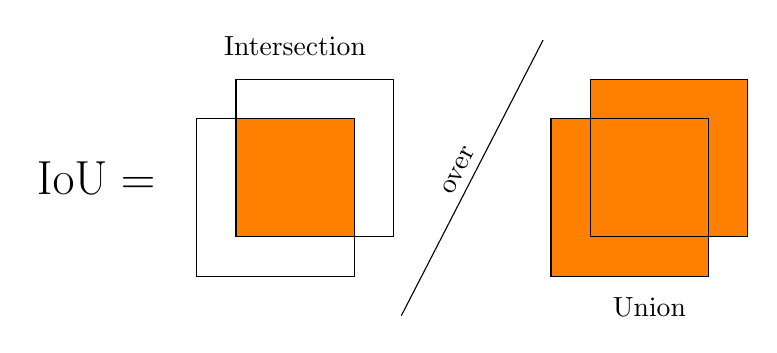
\begin{tikzpicture}
  \node[left] at (-0.4, 1.25) {\LARGE $\mathrm{IoU} = $};
  % Intersection illustration
  \begin{scope}
    \clip (0, 0) rectangle (2, 2);
    \fill[orange] (0.5, 0.5) rectangle (2.5, 2.5);
  \end{scope}
  \draw (0, 0) rectangle (2, 2);
  \draw (0.5, 0.5) rectangle (2.5, 2.5);
  \node[above, yshift=0.5em] at (1.25, 2.5) {Intersection};

  % Division sign
  \draw (2.6, -0.5) -- node[auto, sloped] {over} (4.4, 3);

  % Union illustration
  \begin{scope}[shift={(4.5, 0)}]
    \draw[fill=orange] (0, 0) rectangle (2, 2);
    \draw[fill=orange] (0.5, 0.5) rectangle (2.5, 2.5);
    \draw (0, 0) rectangle (2, 2);
    \node[below, yshift=-0.4em] at (1.25, 0) {Union};
  \end{scope}
\end{tikzpicture}

  \caption{%
    \todo{Write this caption.}
  }%
  \label{fig:iou-metric}
\end{figure}

\begin{figure}[H]
  \centering
  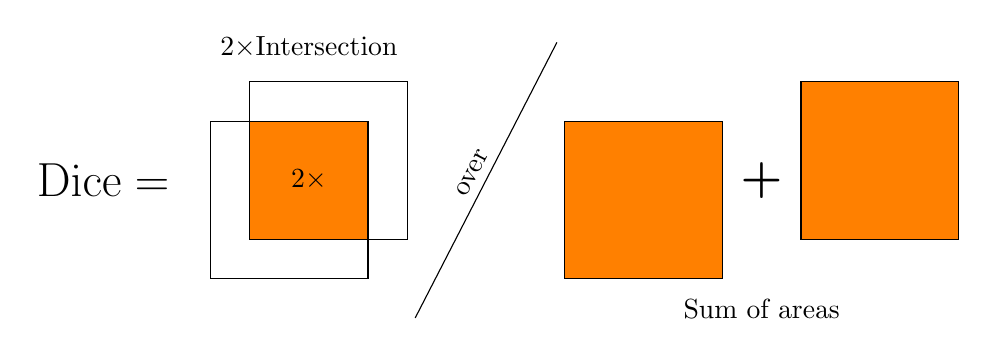
\begin{tikzpicture}
  \node[left] at (-0.4, 1.25) {\LARGE $\mathrm{Dice} = $};

  % Intersection illustration
  \begin{scope}
    \clip (0, 0) rectangle (2, 2);
    \fill[orange] (0.5, 0.5) rectangle (2.5, 2.5);
  \end{scope}
  \draw (0, 0) rectangle (2, 2);
  \draw (0.5, 0.5) rectangle (2.5, 2.5);
  \node[above, yshift=0.5em] at (1.25, 2.5) {$2 \times $Intersection};
  \node at (1.25, 1.25) {$2 \times$};

  % Division sign
  \draw (2.6, -0.5) -- node[auto, sloped] {over} (4.4, 3);

  % Union illustration
  \begin{scope}[shift={(4.5, 0)}]
    \draw[fill=orange] (0, 0) rectangle (2, 2);
    \begin{scope}[shift={(2.5, 0)}]
      \draw[fill=orange] (0.5, 0.5) rectangle (2.5, 2.5);
    \end{scope}
    \draw (0, 0) rectangle (2, 2);
    \node[below, yshift=-0.4em] at (2.5, 0) {Sum of areas};
    \node at (2.5, 1.25) {\LARGE \textbf{+}};
  \end{scope}
\end{tikzpicture}

  \caption{%
    \todo{Write this caption.}
  }%
  \label{fig:dice-coefficient}
\end{figure}


  \topic{Binary cross-entropy and soft dice loss}
  \todo{}

  \todo{}


\subsection{State-of-the-Art}%
\label{sec:state-of-the-art}
At the time of this writing, CNNs have largely surpassed all previous methods for performing image segmentation~\cite{segmentation-overview}, but it is still a relatively new field with constantly new improvements being made.
In the following section we will provide a overview of the current state-of-the-art methods being applied in the field, focusing on what distinguishes these approaches.
Four CNN architectures are considered especially influential as they have become essential building blocks for many segmentation architectures; \textit{AlexNet}, \textit{VGG-16}, \textit{GoogLeNet}, and \textit{ResNet}~\cite{segmentation-overview}.

\textbf{AlexNet}~\cite{segmentation-alexnet} won several image classification competitions when it was first published in~\citeyear{segmentation-alexnet}, including the ILSVRC-2012 competition~\cite{segmentation-overview}.
By employing five convolutional layers, max-pooling layers, ReLU activation functions, and dropout, followed up by a fully-connected feedforward classification network, it outperformed the 2nd place contender by a relatively large margin.

The \textbf{VGG-16} architecture~\cite{vgg-16} published in \citeyear{vgg-16} introduced the idea of stacking several convolution filters with small receptive fields in early layers.
The number of convolution filters are gradually reduced as you move deeper into the network where the receptive fields are larger in size and the resolutions have been reduced.
The result is a network with fewer parameters and more applications of the non-linear activation functions leading to an increased ability to discriminate inputs and reduced training times.
VGG-16 achieved an impressive 92.7\% TOP-5 test accuracy in the ILSVRC-2013 classification competition, inspiring further research involving the techniques employed by the architecture~\cite{segmentation-overview}.

Very deep networks are prone to overfitting and are subject to additional computational overhead.
The \textbf{GoogLeNet} architecture~\cite{googlenet} from \citeyear{googlenet} introduced the \textit{inception module} in order to combat this problem, a building block which allow networks to grow in depth and width with modest increases in computational overhead.
The inception module discards the usual approach of ordering convolutions in a sequential manner, instead opting for several parallel pooled convolution branches with different dimensional properties.
Finally a $1 \times 1$ convolution is applied to each branch in order to reduce the dimensionality of the output and the concatenated result is passed onto the next layer.

The \textbf{ResNet} architecture~\cite{resnet} from \citeyear{resnet} was the result of a continued effort to make deeper architectures feasible.
By training a model with 152 layers ResNet won the ILSVRC-2016 competition with a remarkable 96.4\% accuracy~\cite{segmentation-overview}.

\todo{Remaining topics:}
\begin{itemize}
  \item Recent semantic segmentation progress described here~\cite{segmentation-progress} (\citeyear{segmentation-progress}).
  \item Use of fully convolutional networks for semantic segmentation described here~\cite{segmentation-fcnn} (\citeyear{segmentation-fcnn}).
  \item SegNet architecture described here~\cite{segmentation-segnet} (\citeyear{segmentation-segnet}).
  \item U-Net architecture described here~\cite{segmentation-unet} (\citeyear{segmentation-unet}).
  \item Mask R-CNN architecture described here~\cite{segmentation-mask-r-cnn} (\citeyear{segmentation-mask-r-cnn}).
  \item SegCaps architecture described here~\cite{segmentation-segcaps} (\citeyear{segmentation-segcaps}).
  \item Panoptic feature pyramids described here~\cite{segmentation-panoptic-feature-pyramid} (\citeyear{segmentation-panoptic-feature-pyramid}).
\end{itemize}

